\chapter{Simulator}
\label{chap:sim}

\begin{figure}
	\centering
	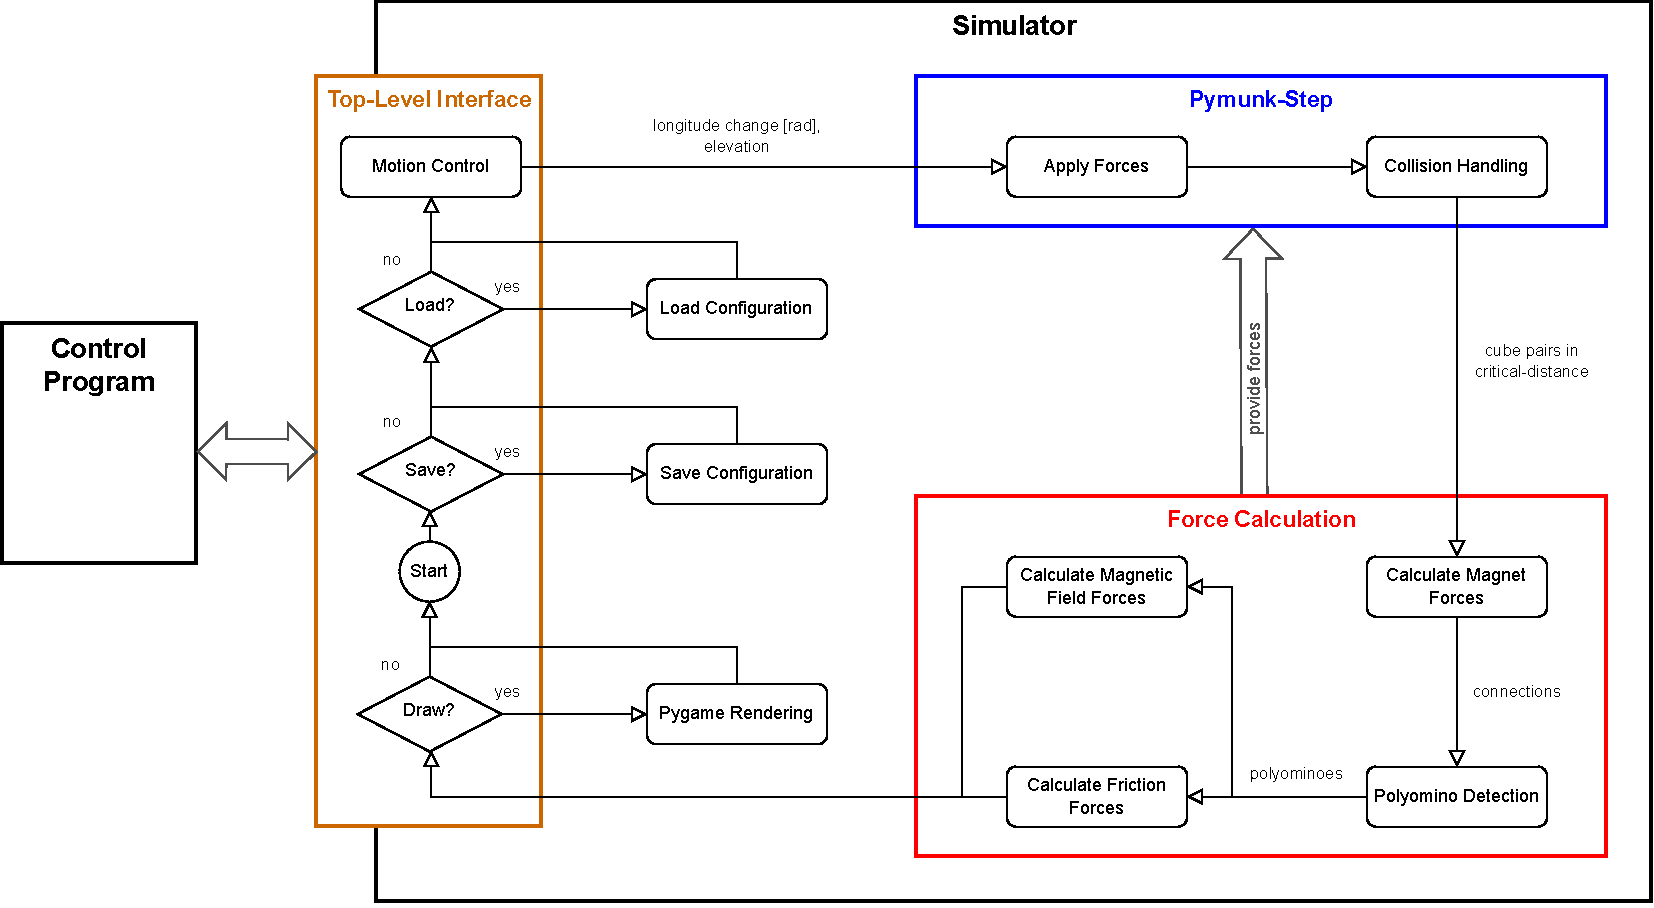
\includegraphics[width=1\textwidth]{figures/simulator_controlflow.pdf}
	\caption[Control flow of the simulator]{Flow chart diagram illustrating the control flow of the simulator's simulation loop. Any control program can interact with the top-level interface of the simulator. Calculated forces are provided to the Pymunk-step for the next iteration of the loop.}
	\label{fig:simulator}
\end{figure}

\begin{figure}
	\centering
	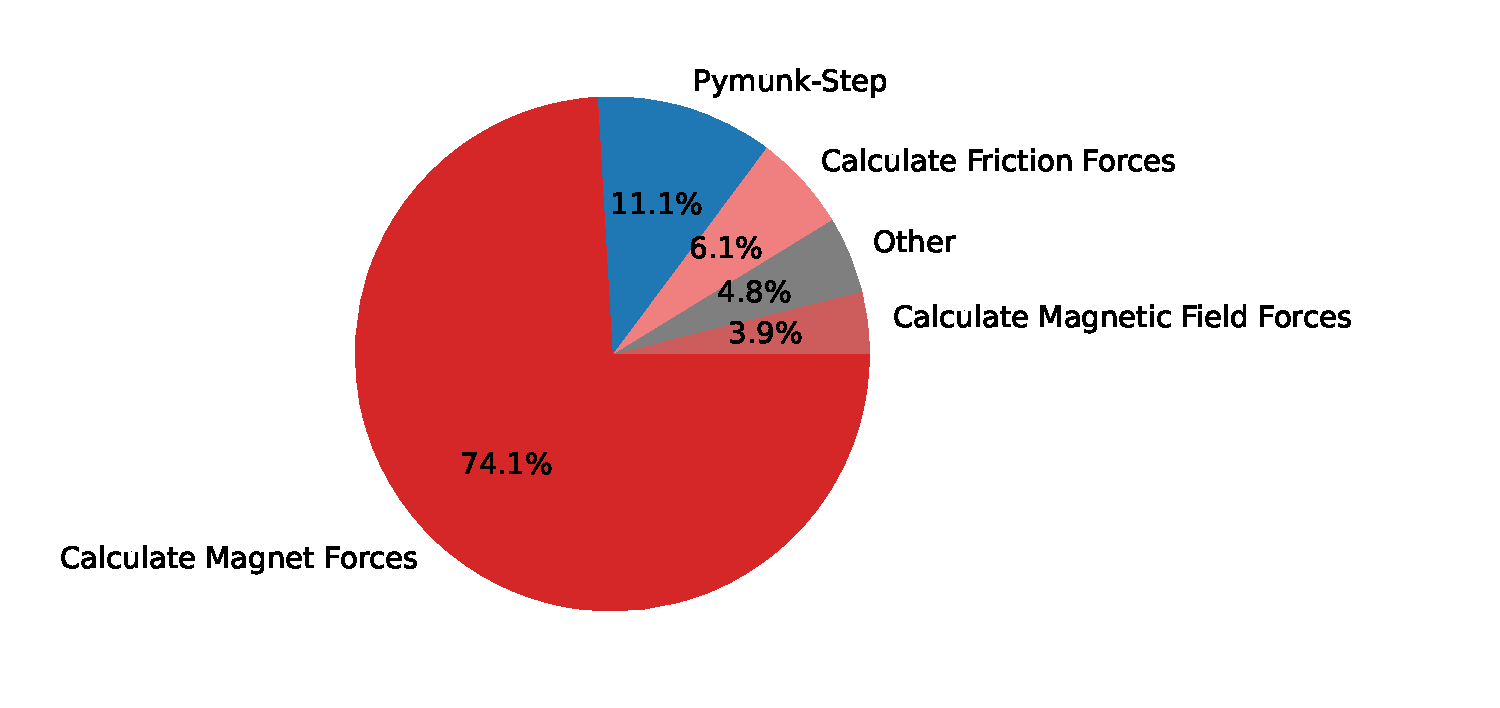
\includegraphics[width=0.9\textwidth]{figures/plots/simulator_timeuse.pdf}
	\caption[Diagram of time-use for certain steps in simulation loop]{Fraction of time used on certain steps in the simulation loop. The simulator ran for $8$ seconds without drawing and executed various motions with ten cubes in the workspace. The steps can be found in the control flow illustrated in \autoref{fig:simulator}.}
	\label{fig:timeuse}
\end{figure}

Our simulator used for modeling the behavior of magnetic modular cubes uses the 2D physics library Pymunk\footnote{Pymunk: \url{https://www.pymunk.org/}}.
This library is build for the Python 3 and Python 2 environment based on the 2D physics library Chipmunk\footnote{Chipmunk: \url{http://chipmunk-physics.net/}}.
We used Pymunk, since it can be easily integrated and customized in a Python implementation.
Furthermore it is light-weight and capable of running headless, but also offers an interface for Pygame\footnote{Pygame: \url{https://www.pygame.org/}}, which we use to visualize developed motion plans and to allow user controls.
As a disadvantage of a 2D simulator, we can only approximate 3D movement, in particular pivot walking.
This way we trade simulation accuracy for faster simulation time, which is necessary to develop global plans in a reasonable time.

In \autoref{fig:simulator} a flow chart diagram illustrates the control flow of the simulator's simulation loop.
The individual steps in the diagram are explained in this and in the following sections.

Any control program, for example a local planner or a ``sandbox program'' for visually controlling magnetic modular cubes with keyboard inputs, can interact with the top-level interface of the simulator.
The interface provides functionalities like starting and stopping the simulation process, controlling the drawing with Pygame, or loading custom configurations and retrieving the current workspace state (\autoref{sec:workspace_state}).
Another crucial functionality is queuing in motions for simulation and notifying the control program when a motion is done simulating.
After handling the motion control, further explained in \autoref{sec:motion_control}, the simulator enters the Pymunk-step.

The Pymunk-step is a library function, responsible for updating the simulation environment by a certain time step.
The duration of a time step is a parameter that allows adjustment between simulation accuracy and simulation time. 
Inside the Pymunk-step forces are applied to the cubes and collision with workspace boundaries and between cubes is handled (\autoref{sec:coll_handling}).

After the Pymunk-step the magnetic forces between the cube's permanent magnets are calculated.
This also determines connections of cube faces that will be used to retrieve information about polyominoes in the workspace (\autoref{sec:force_magnet}).
Polyomino information is necessary to calculate forces of the magnetic field acting on cubes (\autoref{sec:force_field}) and friction forces, on which we heavily rely to simulate 3D movement like pivoting on pivot edges (\autoref{sec:force_friction}).
All the calculated forces will be applied in the Pymunk-step next iteration.

When drawing is enabled, the Pygame-rendering of the workspace is the last step before beginning the next iteration.


\section{Motion Control}
\label{sec:motion_control}

The motion control manages the queued-in motions from the control program and determines a change of the magnetic field for each iteration of the simulation loop.
This change consists of the longitude change in radians and the latitude change called the elevation.
In our simulator the elevation states if the magnetic field lays in the workspace plane, referred to as neutral, or if the magnetic north or south is pointing up.
We do not specify an angular value of the latitude.
The elevation just indicates if polyominoes are pivoting or not.
\autoref{sec:force_friction} has more details.

A change of elevation is executed in a single iteration, but the angle of a rotation will be simulated by multiple longitude changes in a linear ramp with a rotational velocity we choose to set to $\frac{\pi}{8} \, \text{rad}/\text{s}$.
Each motion will be simulated by applying its sequence of updates with a notification to the control program when done.
This makes closed loop control possible, by letting the control program wait until motions are simulated.

Motions control the magnetic field orientation and not the cubes directly.
Cubes will orient themselves by magnetic field forces we further explain in \autoref{sec:force_field}.
The larger a polyomino is, the more time it needs to align with the magnetic field, which can take longer than rotating the magnetic field itself.
A certain amount of zero-updates, dependent on the size of the largest polyomino in the workspace, is added to a rotations update sequence.
This way the control program will not be notified until all polyominoes are aligned with the magnetic field.
This is the reason simulating larger polyominoes requires more simulation time.

%TODO coordinate frame?

\section{Workspace State}
\label{sec:workspace_state}

The state of the workspace is stored and updated within the Pymunk-space.
By saving a configuration of the workspace, relevant attributes like position, orientation and linear and angular velocity of cubes are copied from the Pymunk-space.
When loading in a configuration, the attributes of the Pymunk-space will be manipulated.

Furthermore a configuration stores magnetic field orientation and the polyominoes, together with their center of mass and pivot points.
Polyominoes are stored in a custom data structure that functions both as a list of physical polyominoes and a polyomino set for the use in two-cut-sub-assembly graphs (\autoref{sec:tcsa}).
The data structure and the polyominoes themselves are hash-able for fast equality and inclusion checks.

Individual orientation and velocities of cubes will not be used for planning, but they ensure a correct loading of a workspace configuration that got saved while in motion or when cubes were not or not yet aligned with the magnetic field.
The alignment can be prevented by walls or other cubes, even though we assume perfect alignment with the magnetic field during planning.


\section{Collision Handling}
\label{sec:coll_handling}

Collision is detected and resolved by Pymunk during the Pymunk-step.
For the collision detection Pymunk uses a bounding volume hierarchy of objects in the Pymunk-space.
We make use of this efficient collision detection for determining cube pairs in critical-distance.
For that, each cube is surrounded by a circular sensor with a radius of half the critical-distance.
A cube pair is in critical-distance if their sensors collide.
We set the critical-distance to $5 r_C$.
More on the use of cube pairs in critical-distance in \autoref{sec:force_magnet}.

\section{Simulating Forces}

To model accurate behavior of magnetic modular cubes we calculate and apply the three most significant forces acting on cubes in the workspace.
The reason forces are calculated after the Pymunk-step, where they are applied, is because of the cube pairs in critical-distance determined with the collision detection of Pymunk.
Providing forces for the appliance in the next iteration does not effect simulation accuracy.

\subsection{Magnet Forces}
\label{sec:force_magnet}

\begin{figure}
	\centering
	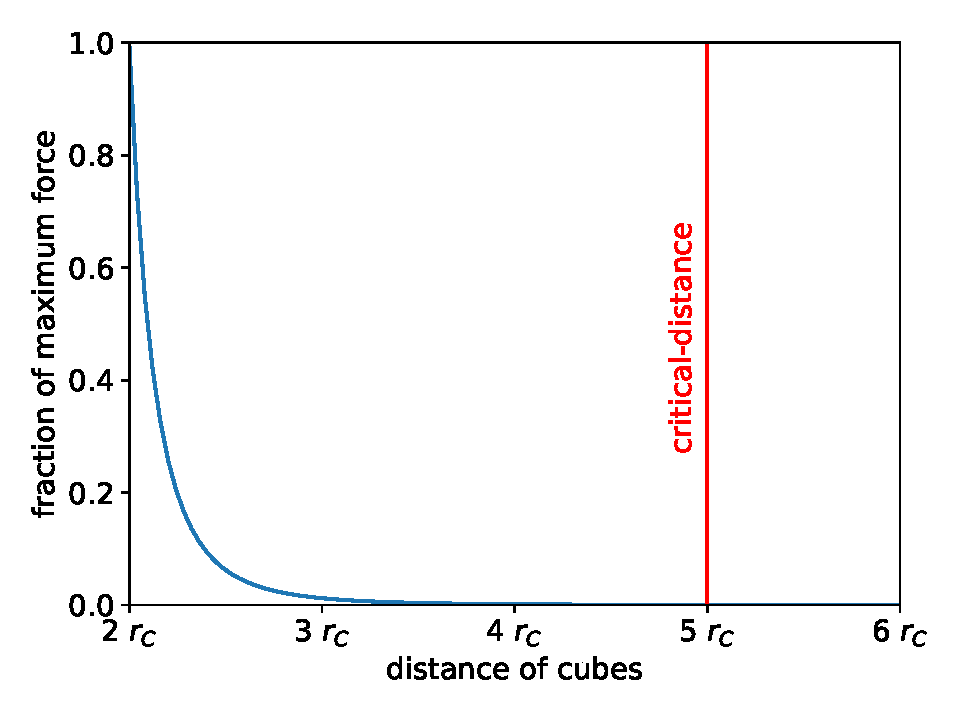
\includegraphics[width=0.6\textwidth]{figures/plots/magnet_force.pdf}
	\caption[Declining magnetic forces with increasing cube distance.]{Decline of magnetic force between two permanent magnets with increasing distance between the cube centers. We reach a maximum force at $2 r_C$, when the cube faces are in contact. With distances bigger than the critical-distance of $5 r_C$ the fraction of force is negligible.}
	\label{fig:magnet_force}
\end{figure}

The magnetic dipole-dipole interaction of permanent magnet is the driving force for self-assembly.
Cubes attract and repulse each other, which results in connection of cube faces and therefore the construction of polyominoes.
In our simulator nothing more than magnet force is responsible for keeping cubes connected, as it would be in a real world application of magnetic modular cubes.
Nevertheless, fast rotation or hitting workspace boundaries can cause connections to break.

We can define a maximum attraction force when cubes are at a distance of $2 r_C$.
When such a force is reached with a valid pair of cube faces we mark the faces as connected.
Based on the marked connections polyominoes in the workspace can be identified.

The majority of simulation time, about $75\%$, is spend on calculating magnet forces as shown in \autoref{fig:timeuse}.
Cubes not in critical-distance are to far away to significantly affect each other with magnetic forces of their permanent magnets.
The steep decline of magnetic force with increasing cube distance can be seen in \autoref{fig:magnet_force}.
We only calculate magnet forces for cube pairs in critical-distance to speed up simulation.
Because assembling large target shapes is the goal of global planning, it is not uncommon that most cubes are in critical-distance.
For a more efficient simulation we further determine which magnet pairs to consider.

\paragraph{Determining Magnet Pairs}

For a single cube pair each of the four magnets of one cube interacts with each magnet of the other cube, resulting in $16$ magnet pairs to consider for a physically accurate simulation.
Magnet forces of pairs within the same cube are neglected, since they do not result in any movement.
Determining the first $k$ pairs with minimal distance is a reasonable approach to not calculate all $16$ pairs, since they should have the strongest force interaction.
Of course $k=1$ is most efficient, but results in a loss of real world behavior of magnetic modular cubes.
We choose $k=4$ to again find balance between accuracy and efficiency.

\paragraph{Calculating Magnet Force}

Each calculated force of a magnet pair is applied at the position of both magnets in opposite direction, resulting in either attraction or repulsion.
For two magnets with moments $m_1$ and $m_2$ and a distance of $r$ the magnet force acting from magnet 1 on magnet 2 is
\begin{equation}
F_\textit{mag} = \frac{\mu_\textit{mag}}{r^4} \left(m_2(m_1 \cdotp \hat{r}) + m_1(m_2 \cdotp \hat{r}) + \hat{r}(m_1 \cdotp m_2) - 5\hat{r}(m_1 \cdotp \hat{r})(m_2 \cdotp \hat{r}) \right) \, ,
\end{equation}
with $\hat{r}$ being the unit vector pointing from magnet 1 to magnet 2.
The force acting from magnet 2 on magnet 1 is $-F_\textit{mag}$.
We set the strength of all magnets to $\mu_\textit{mag} = 2.5 \cdot 10^7$ \cite{levitt2013}. 


\subsection{Magnetic Field Forces}
\label{sec:force_field}

Magnetic field forces are responsible for aligning cubes with the longitude orientation of the magnetic field.
Force is applied only at the position of north and south magnets for each cube of a polyomino.
The forces at north and south magnets act in opposite directions to ensure a rotation.
$F_\textit{field}$ is calculated based on the difference of cube orientation $\gamma_\textit{cube}$ and magnetic field orientation $\gamma_\textit{field}$ with
\begin{equation}
F_\textit{field} = \mu_\textit{field} \begin{pmatrix} \sin(\gamma_\textit{cube} - \gamma_\textit{field}) \\ 0 \end{pmatrix} \mathbf{R}_{\gamma_\textit{cube}} \, .
\end{equation}
$\mu_\textit{field} = 1000$ is the strength of the magnetic field and $\mathbf{R}_{\gamma_\textit{cube}}$ is the rotation matrix used for rotating the force direction by $\gamma_\textit{cube}$.
An alignment where $\gamma_\textit{cube} = \gamma_\textit{field}$ results in $F_\textit{field} = \vec{0}$.


\subsection{Friction Forces}
\label{sec:force_friction}

Since we are working with a 2D-simulation, a workaround is needed to simulate pivoting of polyominoes.
In the simulator a pivoting polyomino changes its center of rotation from the center of mass to either the north or the south pivot point.
To archive this, friction forces are applied at different points depending on the three states of magnetic field elevation specified in \autoref{sec:motion_control}.

Friction forces are applied per cube at a friction-point $p_\textit{fric}$, but polyomino information is still necessary to determine cubes that are in contact with the ground, called friction-cubes.
In case of a neutral elevation, all cubes of the polyomino are friction-cubes and $p_\textit{fric}$ is the cube center.
If the magnetic north is pointing up, all cube along the south pivot-edge become friction-cubes and $p_\textit{fric}$ becomes the position of the south magnet.
If the magnetic south is pointing up, all cube along the north pivot-edge are friction-cubes with $p_\textit{fric}$ being the position of the north magnet.
The force applied for friction-cubes is dependent on the velocity at the friction-point $v_{p_\textit{fric}}$ and the mass of a cube $m_C$
\begin{equation}
F_\textit{fric} = -v_{p_\textit{fric}} \cdot m_C \cdot \frac{n}{n_\textit{fric}} \, .
\end{equation}
$n$ is the size of the polyomino and $n_\textit{fric}$ the number of friction cubes.
The force is divided by $n_\textit{fric}$, so that $F_\textit{fric}$ is distributed equally on each friction-cube.
Multiplying by $n$ accounts for the mass of all cubes in the polyomino, which is carried by the friction-cubes.

To ensure a more stable simulator, we apply a nominal friction force
\begin{equation}
F_\textit{nom} = -v_{p_\textit{fric}} \cdot m_C \cdot w_\textit{nom}
\end{equation}
to all non friction-cubes.
We control the fraction of this force by $w_\textit{nom} = 0.35$.


